\chapter{Θεωρητική ανάλυση}

\section{Εισαγωγή}
Σε αυτό το κεφάλαιο θα γίνει μια σύντομη ανάλυση εννοιών οι οποίες είναι αναγκαίο να γίνουν κατανοητές προτού εισέλθουμε σε λεπτομερείς ανάλυση της πτυχιακής εργασίας. Επιπλέον, θα γίνει σύντομη ανάλυση των απαιτήσεων για την επίτευξη της πτυχιακής όπως επίσης και των εργαλείων που χρησιμοποιήθηκαν. 

\section{Ανάπτυξη εφαρμογών κινητών συσκευών}
Όπως είναι γνωστό, η εξέλιξη της τεχνολογίας στο τομέα των κινητών συσκευών είναι ραγδαία τα τελευταία χρόνια με αποτέλεσμα οι δυνατότητες τους συνεχώς να επεκτείνονται. Πλέον μια συσκευή παρέχει στο χρήστη δυνατότητες αντάξιες ενός υπολογιστή σε ένα αισθητά πολύ μικρότερο μέγεθος. Εδώ θα πρέπει να σημειώσουμε ότι ο όρος κινητές συσκευές δεν διαχωρίζει τις τηλεφωνικές συσκευές από τα tablet καθώς ο διαχωρισμός μεταξύ τους, την σήμερον ημέρα, γίνεται όλο και πιο δύσκολος. Παρακάτω θα αναλύσουμε τις εφαρμογές κινητών συσκευών, την ιστορική αναδρομή των τελευταίων ετών καθώς και τις κύριες πλατφόρμες που βρίσκονται αυτή τη στιγμή στην αγορά. Επίσης θα αναλύσουμε τα προβλήματα τα οποία εμφανίζει η σημερινή αγορά κινητών συσκευών σε έναν προγραμματιστή και τις λύσεις που προσφέρονται.

\subsection{Εξέλιξη στον τομέα των κινητών συσκευών}
Οι κινητές συσκευές είχαν μια συνεχή εξέλιξη από τις αρχές του 2000 με καινούριες δυνατότητες να προστίθενται συνεχώς και η λειτουργικότητα τους να αυξάνεται αισθητά. Εάν επικεντρωθούμε στα νεότερα χρόνια, Από την εμφάνιση του πρώτου iPhone το 2007 της εταιρείας Αpple η οποία έκανε το πρώτα βήματα στον κόσμο των έξυπνων τηλεφώνων (smartphones), μέχρι την εμφάνιση του android λειτουργικού συστήματος μπορούμε να παρατηρήσουμε πως οι κατασκευάστριες εταιρείες επικεντρώνονται όλο και περισσότερο στην αύξηση των δυνατοτήτων που μπορεί να προσφέρει μια κινητή συσκευή. 
\par
Εν έτη 2018 μία απλή κινητή συσκευή έχει εξίσου τις ίδιες δυνατότητες με έναν ηλεκτρονικό υπολογιστή. Ο χρήστης έχει τη δυνατότητα σύνδεσης στο διαδίκτυο, την χρήση πολύπλοκων εφαρμογών όπως λογισμικά επεξεργασίας κειμένου μέχρι τη χρήση εφαρμογών GPS για τη καθοδήγηση του. Θα τολμούσαμε να πούμε πως καθημερινά το χάσμα μεταξύ των ηλεκτρονικών υπολογιστών και των κινητών συσκευών γίνεται όλο και μικρότερο.

\subsection{Πλατφόρμες κινητών συσκευών}
Ακολουθώντας την εξέλιξη στις κινητές συσκευές, παρατηρούμε ότι διάφορες πλατφόρμες και λειτουργικά συστήματα έχουν κάνει την εμφάνιση τους. Σκοπός της εργασίας αυτής δεν είναι να αναλύσει τις διάφορες πλατφόρμες, παρόλα αυτά είναι αναγκαία η παρουσίαση τους στον αναγνώστη για την περαιτέρω κατανόηση της ανάπτυξης της εφαρμογής. Σήμερα οι μεγαλύτερες πλατφόρμες κινητών συσκευών στην αγορά είναι τρεις:

\begin{description}
\item [iOs] Είναι το λειτουργικό σύστημα στις συσκευές iphone και ipad της εταιρείας Apple.

\item [Windows phone] Είναι το λειτουργικό σύστημα της εταιρείας Microsoft. Κάνει την εμφάνιση του κυρίως στις συσκευές της εταιρείας Nokia.

\item [Android] Είναι το λειτουργικό σύστημα ανοιχτού κώδικα της εταιρείας Google. Εμφανίζεται σε διάφορες συσκευές διάφωρων εταιρειών. Θεωρείται το κυρίαρχο λειτουργικό σύστημα στην αγορά εργασίας.
\end{description}

\par
Φυσικά υπάρχει ένα αξιοσέβαστος αριθμός άλλων λειτουργικών συστημάτων που έχουν κάποιο μερίδιο στην αγορά. Η παραπάνω επιγραμματική παρουσίαση έχεις ως στόχο να προσφέρει στον αναγνώστη μια μικρή εισαγωγή στο πρόβλημα που αντιμετωπίζουν οι προγραμματιστές εφαρμογών κινητών συσκευών. Κάθε πλατφόρμα χρησιμοποιεί διαφορετικές γλώσσες προγραμματισμού με αποτέλεσμα η ανάπτυξη εφαρμογών να είναι ένα καίριο ζήτημα για τον προγραμματιστή. Με ποιον τρόπο επιλέγεις την πλατφόρμα ανάπτυξης και αν θελήσεις να υποστηρίξεις περισσότερο από μία, ποιο θα είναι το κόστος ανάπτυξης όπως επίσης και το κόστος συντήρησης;

\subsection{Υβριδικές εφαρμογές}
Καθώς οι διάφορες πλατφόρμες εξελίσσονται συνεχώς, αυτομάτως, καθίσταται μεγάλη πρόκληση η ανάπτυξη μιας εφαρμογής συμβατή με όλα τα διαφορετικά λειτουργικά συστήματα. Στην πραγματικότητα ο προγραμματιστής είναι αναγκασμένος να αναπτύξει την ίδια εφαρμογή πολλαπλές φορές. Αυτομάτως αυτή η κατάσταση αυξάνει το κόστος συντήρησης ακόμη και μιας απλής εφαρμογής.
\par 
Για την αντιμετώπιση του παραπάνω προβλήματος δημιουργήθηκαν κατάλληλα εργαλεία τα οποία προσφέρουν στον προγραμματιστή τη δυνατότητα ανάπτυξης της εφαρμογής μια φορά και να τη καθιστά συμβατή με τις περισσότερες κυρίαρχες πλατφόρμες. Ένα εργαλείο το οποίο προσφέρει αυτές τις δυνατότητες είναι το Apache Cordova framework. 

\subsubsection{Apache Cordova}
Κάνοντας χρήση του Cordova framework, o προγραμματιστής αναπτύσσει την εφαρμογή του με τεχνολογίες διαδικτύου όπως HTML, CSS, JavaScript. Η πλατφόρμα Cordova δίνει στο προγραμματιστή πρόσβαση στις δυνατότητες της κάθε συσκευής (κάμερα, GPS κ.τ.λ), ανεξαρτήτων λειτουργικού συστήματος, μέσα από μια ενοποιημένη διεπαφή \citep{Cordova} \citep{CordovaWiki}. Έτσι η εφαρμογή μπορεί να εκτελεστεί στα διάφορα λειτουργικά συστήματα. Παρόλα αυτά το Cordova framework έχει σαν μοναδικό στόχο τον παραπάνω, με αποτέλεσμα να μην ασχολείται καθόλου με την αισθητική και εμφάνιση της εφαρμογής.

\subsubsection{Ionic Framework}
Το Ionic framework προσφέρει στο προγραμματιστή τα απαραίτητα εξαρτήματα για τη δημιουργία μιας διεπαφής χρήστη η οποία ακολουθεί τα πρότυπα κάθε πλατφόρμας \citep{Ionic} \citep{IonicWiki}. Με αυτό το τρόπο ο προγραμματιστής σχεδιάζει τη διεπαφή χρήστη με αισθητική αποδεκτή από όλους τους χρήστες ανεξαρτήτως της πλατφόρμας επιλογής τους.

\subsubsection{Cordova \& Ionic}
Ο συνδυασμός των Cordova και Ionic frameworks προσφέρει στο προγραμματιστή ένα πλήρες σύστημα για τη δημιουργία υβριδικών εφαρμογών. Εδώ να σημειώσουμε πως τα παραπάνω εργαλεία δεν είναι τα μοναδικά στην αγορά, παρόλα αυτά θεωρούνται τα πιο ώριμα και προσφέρουν περισσότερες δυνατότητες σε σύγκριση με άλλα.

\section{Ανάπτυξη εφαρμογών διαδικτύου}
Οι ιστοσελίδες πλέον δεν παρουσιάζουν απλά ένα στατικό περιεχόμενο αλλά προσφέρουν στο χρήστη διαδραστικό περιεχόμενο. Η ραγδαία αύξηση των χρηστών στο χώρο του διαδικτύου δημιούργησε την ανάγκη ανάπτυξης προηγμένων ιστοσελίδων οι οποίες προσφέρουν στους χρήστες περισσότερες και πιο σύνθετες δυνατότητες. Σταδιακά όλες οι υπηρεσίες μεταφέρονται στο διαδίκτυο. Από ηλεκτρονικά καταστήματα αγορών μέχρι πολυσύνθετες εφαρμογές όπως κρατικές υπηρεσίες. Το φαινόμενο αυτό είχε ως αποτέλεσμα την ανάγκη νέων εργαλείων τα οποία μπορούν να προσφέρουν στο προγραμματιστή τη δυνατότητα ανάπτυξης αυτού του είδους εφαρμογών. Ένα από τα πιο ισχυρά εργαλεία στην αγορά είναι το AngularJS framework.

\subsubsection{AngularJS Framework}
Το AngularJS framework είναι ένα εργαλείο κατασκευής εφαρμογών διαδικτύου. Προσφέρει στον προγραμματιστή τη δυνατότητα να χειριστεί το περιεχόμενο της εφαρμογής του με δυναμικό τρόπο \citep{AngularJS} \citep{AngularJSWiki}. Με αυτό το τρόπο ο προγραμματιστής μπορεί να κατασκευάσει μία εφαρμογή διαδικτύου που είναι ικανή να προσφέρει τις ίδιες δυνατότητες με μία εφαρμογή ηλεκτρονικών υπολογιστών.

\section{Web Services}
Web Service είναι μια υπηρεσία η οποία είναι προσβάσιμη μέσω του διαδικτύου με στόχο την εξυπηρέτηση των χρηστών της ή άλλων εφαρμογών. Το web service καταστεί δυνατή την επικοινωνία διαφορετικών πελατών μέσω του HTTP πρωτοκόλλου. To web service προσφέρει πρόσβαση στις υπηρεσίες του μέσω ενός API. Η επικοινωνία γίνεται μέσω αιτήσεων, δηλαδή ο πελάτης ζητάει κάτι, το web service επεξεργάζεται το αίτημα και επιστρέφει την κατάλληλη απάντηση. Τα σύγχρονα web services χρησιμοποιούν την αρχιτεκτονική ReST για την υλοποίηση των API τους.

\begin{figure}[h]
  \centering
  \includegraphics[width=110mm]{images/web-service.png}
  \caption{Παράδειγμα Επικοινωνίας web service}
  \label{fig:web-service}
\end{figure}

\subsection{ReST API}
Όπως αναφέραμε παραπάνω το ReST είναι μία αρχιτεκτονική σχεδιασμού και υλοποίησης διεπαφών μεταξύ πελατών και web services. Χρησιμοποιεί το πρωτόκολλο HTTP ως δίαυλο επικοινωνίας. Λειτουργεί ανεξαρτήτως πλατφόρμας και γλώσσας προγραμματισμού οπότε καθιστά δυνατή την εξυπηρέτηση διαφορετικών πελατών. Η αρχιτεκτονική ReST βασίζεται σε 6 βασικές αρχές \citep{ReST}:

\subsubsection{Πελάτη-Εξυπηρετητή}
Το σύστημα είναι της μορφής πελάτη-εξυπηρετητή. Οι πελάτες είναι υπεύθυνοι για την εκκίνηση της επικοινωνίας καθώς ο εξυπηρετητής περιμένει για αιτήματα. Με αυτό το τρόπο οι ρόλοι διαχωρίζονται και η επικοινωνιακές αρχές είναι διακριτές.

\subsubsection{Πολυεπίπεδο σύστημα}
Το σύστημα διαχωρίζεται σε πολλαπλά επίπεδα με το κάθε επίπεδο να εξυπηρετεί το αμέσως επόμενο. Έτσι τα διάφορα επίπεδα παραμένουν αόρατα μεταξύ τους και το κάθε επίπεδο γνωρίζει μονάχα για το αμέσως επόμενο. 

\subsubsection{Stateless}
Κάθε αίτημα πρέπει να είναι ανεξάρτητο. Ο πελάτης είναι υπεύθυνος να προσφέρει όλες τις απαιτούμενες πληροφορίες στο εξυπηρετητή σε κάθε αίτημα του. Με αυτό το τρόπο ο εξυπηρετητής προσφέρει τις υπηρεσίες του ανεξαρτήτως άλλων αιτήσεων.

\subsubsection{Cacheable}
Το κάθε επίπεδο έχει τη δυνατότητα αποθήκευσης στη μνήμη οποιασδήποτε απάντησης έχει λάβει από κάποιο άλλο επίπεδο. Έτσι ο όγκος δεδομένων ελαττώνεται σημαντικά.

\subsubsection{Code on demand}
Ο πελάτης έχει τη δυνατότητα να αιτηθεί κομμάτια κώδικα τα οποία μπορεί να εκτελέσει για να επιτευχθεί κάποιος στόχος. Παραδείγματα τέτοιου κώδικα είναι ο JavaScript κώδικας που εκτελείται σε μία ιστοσελίδα.

\subsubsection{Ομοιόμορφη διεπαφή}
Η επικοινωνία μεταξύ πελάτη και εξυπηρετητή οφείλει να ακολουθεί κάποιες βασικές αρχές και πρότυπα ώστε η επικοινωνία να είναι δυνατή και να μην καταρρεύσει.

\begin{figure}[h]
  \centering
  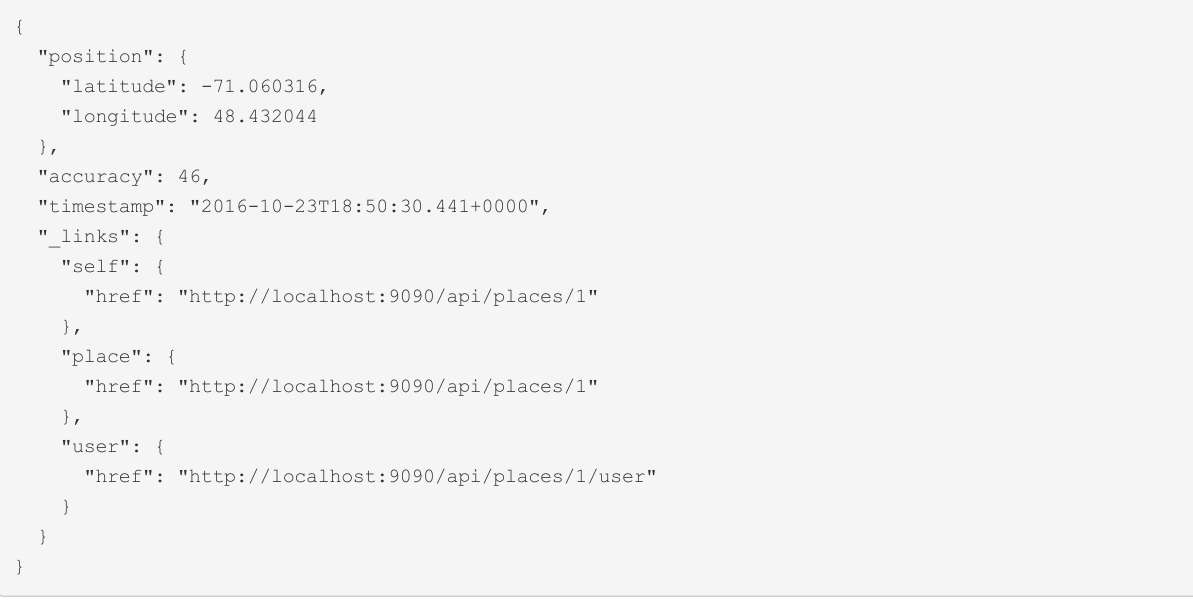
\includegraphics[width=140mm]{images/request.png}
  \caption{Παράδειγμα απάντησης σε JSON μορφή}
  \label{fig:request}
\end{figure}

Για να γίνουν αντιληπτά τα παραπάνω στο διάγραμμα ~\ref{fig:request} εμφανίζεται ένα απλό παράδειγμα απάντησης ενός εξυπηρετητή που χρησιμοποιεί ReST API. Ο πελάτης χρησιμοποιώντας το HTTP πρωτόκολλο έκανε μία αίτηση στο URL:

\textbf{http://servername.com/api/places/1}

ζητώντας να του επιστραφούν οι πληροφορίες της περιοχής με ταυτότητα 1.

\subsection{Websockets}
Όπως αναφέραμε παραπάνω ένα ReST API βασίζεται στην αρχή αίτησης-απάντησης με αποτέλεσμα ο πελάτης να είναι αναγκασμένος να δημιουργεί πολλαπλά αιτήματα. Η μέθοδος αυτή λειτουργεί σε περιπτώσεις που ο πελάτης δεν έχει την ανάγκη να λαμβάνει άμεσα οποιαδήποτε αλλαγή στα δεδομένα τα οποία των απασχολούν 
. Υπάρχουν όμως περιπτώσεις στις οποίες η επικοινωνία μεταξύ πελάτη και εξυπηρετητή πρέπει να είναι αμφίδρομη. Υπάρχουν σενάρια στα οποία ο εξυπηρετητής πρέπει να ενημερώνει τον πελάτη χωρίς την ανάγκη δημιουργίας ενός νέου αιτήματος. Για την επίλυση του παραπάνω προβλήματος μπορεί να γίνει χρήση των websocket.
\par
Το websocket είναι ένα πρωτόκολλο τυποποιημένο από τον οργανισμό IETF \citep{websockets}. Καθιστά δυνατή τη πλήρη αμφίδρομη επικοινωνία μεταξύ πελάτη και εξυπηρετητή στο επίπεδο του TCP. Η αρχική επικοινωνία μεταξύ πελάτη και εξυπηρετητή επιτυγχάνεται μέσω HTTP. Εφόσον η επικοινωνία θεωρηθεί επιτυχείς το πρωτόκολλο αναβαθμίζεται σε websocket. Έτσι δημιουργείται ένας αγωγός μεταξύ πελάτη και εξυπηρετητή ο οποίος μπορεί να χρησιμοποιηθεί και από τους δύο.

\begin{figure}[h]
  \centering
  \includegraphics[width=140mm]{images/websocket.png}
  \caption{Παράδειγμα επικοινωνίας μέσω websocket}
  \label{fig:websocket}
\end{figure}

\newpage

\subsection{Publish-Subscribe}
Publish-subscribe είναι ένα μοτίβο αποστολής μηνυμάτων στο οποίο οι αποστολείς δεν στέλνουν τα μηνύματα τους άμεσα στους αποδέκτες, αλλά αποστέλλονται σε ένα διαμεσολαβητή ο οποίος είναι υπεύθυνος για τη δρομολόγησή τους \citep{publishSubscribeWiki}. Ένα απλό παράδειγμα βιβλιοθήκης η οποία επιτρέπει τη χρήση του μοτίβου publish-subscribe μέσω του websocket πρωτοκόλλου είναι η βιβλιοθήκη Stomp. Ο τρόπος λειτουργίας όπως εμφανίζεται στο διάγραμμα ~\ref{fig:publish-subscribe} είναι ο εξής:

\begin{itemize}
\item Δημιουργείται ένα θέμα το οποίο μπορεί να απασχολεί τους χρήστες (topic).
\item Οι χρήστες οι οποίοι ενδιαφέρονται για το παραπάνω θέμα γίνονται συνδρομητές πάνω σε αυτό (subscribe).
\item Κάποιος από τους χρήστες στέλνει κάποιο μήνυμα στο παραπάνω θέμα (publish).
\item Τέλος οι συνδρομητές που έχουν εγγραφεί στο παραπάνω θέμα λαμβάνουν το μήνυμα που δημοσιεύθηκε.
\end{itemize}


\begin{figure}[h]
  \centering
  \includegraphics[width=120mm]{images/publish-subscribe.png}
  \caption{Παράδειγμα publish-subscribe}
  \label{fig:publish-subscribe}
\end{figure}

\subsection{Spring Framework}
Από τις παραπάνω πληροφορίες είναι φανερή η ανάγκη εύρεσης ενός εργαλείου το οποίο θα βοηθήσει στην ανάπτυξη του web service. Ένα από τα πιο ισχυρά εργαλεία είναι το Spring Framework. Το Spring framework χαρακτηρίζεται ως ένα application framework το οποίο εξυπηρετεί στην δόμηση της εφαρμογής \citep{springframework}. Στο συγκεκριμένο σύστημα χρησιμοποιήθηκε στη δημιουργία ενός σύνθετου εξυπηρετητή ο οποίος θα μπορεί να παρέχει υπηρεσίες στους πελάτες του. Έτσι με τη βοήθεια του Spring framework ήταν δυνατή η δημιουργία ενός εξυπηρετητή που παρέχει ένα ReST API καθώς και τη δυνατότητα publish-subscribe μέσω websockets.
